\section{Results}

\subsection{Speed}
\begin{table}[H]
  \centering
  \caption{Time to open the \SI{7.6}{\giga\byte}, \SI{4.7}{\hour} recording (Mac, 8 cores, 4 workers).}
  \label{tab:speed}
  \begin{tabular}{lrr}
    \toprule
    Step & First open (s) & Next open (s) \\
    \midrule
    CSV $\rightarrow$ \SI{1}{\kilo\hertz} & 9.1 & 0.04 \\
    Part A & 0.6 & 0.02 \\
    Part B & 1.1 & 1.1 \\
    \midrule
    Total & 10.8 & 1.2 \\
    \bottomrule
  \end{tabular}
\end{table}
The first open takes \SI{10.8}{\second}. After
that, the 1\,kHz signal and the Part A result come from the cache, so the file opens in
\SI{1.2}{\second}. The results are the same with and without the cache.

\subsection{Detection results}
\label{sec:detection-results}
\subsubsection{Big pieces}
Every piece was found (Table~\ref{tab:bigpieces},
Figure~\ref{fig:detection}); in the high section two pieces were split in two, giving 17. 41 of
the 45 dyed pieces were labelled \texttt{dyed}; the other pieces in these sections were below the
no-dye level and labelled \texttt{solid\_no\_dye}, so all were counted as tissue. No no-dye piece
was labelled \texttt{dyed}. However, all 4 water events after the tissue passed the two-channel check and were labelled \texttt{solid\_no\_dye}.
In the water-only recording, 1 of 39 events reached the no-dye level.

\begin{table}[H]
  \centering
  \caption{Labels in the Big pieces recording, by section.}
  \label{tab:bigpieces}
  \begin{tabular}{lrrrr}
    \toprule
    Section & Events & \texttt{dyed} & \texttt{solid\_no\_dye} & \texttt{water} \\
    \midrule
    High & 17 & 13 & 4 & 0 \\
    Middle & 15 & 14 & 1 & 0 \\
    Low & 15 & 14 & 1 & 0 \\
    Zero (no dye) & 15 & 0 & 15 & 0 \\
    Water & 4 & 0 & 4 & 0 \\
    \bottomrule
  \end{tabular}
\end{table}

\begin{figure}[H]
  \centering
  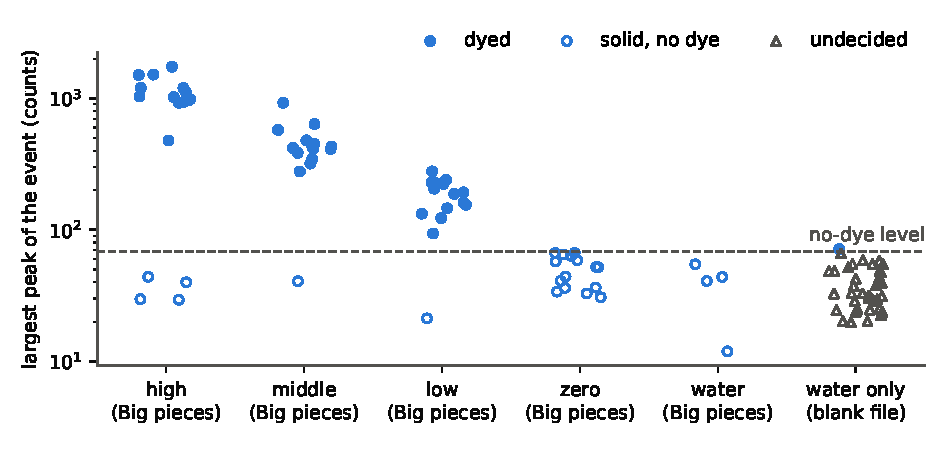
\includegraphics[width=\linewidth]{img/fig_detection.pdf}
  \caption{Largest peak of each event. In the water-only recording \texttt{adc1} hardly
           responds, so dim events are \texttt{undecided}.}
  \label{fig:detection}
\end{figure}

\subsubsection{All recordings}
The pipeline ran to the end on all 29 recordings
(Table~\ref{tab:allrecordings}). In the 28 recordings where \texttt{adc1} responds, the chance
rate was at most 15\,\% (median 5\,\%), so the two-channel check was used in all of them, and 82\,\%
of the \texttt{dyed} pieces also passed the check (62--100\,\% per recording).

\begin{table}[H]
  \centering
  \caption{Events and labels in all recordings.}
  \label{tab:allrecordings}
  \begin{tabular}{lrrrrrr}
    \toprule
    Group & Files & Events & \texttt{dyed} & No dye & Water & Undecided \\
    \midrule
    Big pieces & 1 & 69 & 41 & 26 & 2 & 0 \\
    Water only & 1 & 39 & 1 & 0 & 0 & 38 \\
    Known volumes (2025) & 9 & 246 & 176 & 16 & 54 & 0 \\
    Tumour & 10 & 285 & 241 & 21 & 23 & 0 \\
    Demo sessions & 8 & 377 & 187 & 112 & 78 & 0 \\
    \bottomrule
  \end{tabular}
\end{table}

\subsubsection{Comparison with simpler methods}
To see what the two less obvious steps add, we ran the same recordings with a simpler version of
each step and everything else unchanged (\texttt{tools/benchmark\_methods.py};
Table~\ref{tab:simple}). For $\sigma$, the simple version uses all \SI{200}{\milli\second}
blocks, including the idle ones. For the two-channel check, it looks for any \texttt{adc1} peak
within \SI{\pm 20}{\milli\second} of the largest \texttt{adc2} peak, without the lag correction
and the 5\,\% height condition.

\begin{table}[H]
  \centering
  \caption{Current and simple methods on the same recordings. Only the named step differs.}
  \label{tab:simple}
  \begin{tabular}{llrr}
    \toprule
    Step & Result & Current & Simple \\
    \midrule
    $\sigma$ & events in the 29 recordings & 1016 & 876 \\
             & events in one demo recording & 48 & 1 \\
    Two-channel check & chance rate, median / max & 5 / 15\,\% & 7 / 40\,\% \\
             & recordings where the check is used & 28 of 28 & 27 of 28 \\
             & \texttt{dyed} pieces also confirmed & 82\,\% & 70\,\% \\
    \bottomrule
  \end{tabular}
\end{table}

With all blocks, idle periods make $\sigma$ too small. The threshold then falls below the water
wiggles, and separate pieces join: in one demo recording with long idle periods all 48 events
became one. With the simple two-channel check, small \texttt{adc1} noise peaks pass more often
by chance; in the \SI{4.7}{\hour} recording the chance rate reached 40\,\%, so the check could
not be used there, and fewer dyed pieces were confirmed. In the Big pieces recording, both
simple versions gave the same labels as the current ones, so the gain shows only in the
other recordings.


\subsection{Amount of tissue}
\label{sec:amount-results}
When the concentration is known, the area scales with the amount with an error of 15--21\,\%
(Table~\ref{tab:amount}, Figure~\ref{fig:amount}). But \SI{1}{\milli\litre} of high
concentration gives 3.2 times the area of middle (dye ratio 4.8), so with one $k$ for both the
error rises to 68\,\%. A re-suction gives 0.5--0.7 times the area of the first suction.
With only four or five recordings per group, the 95\,\% prediction interval for a new recording
is wide: a factor of 1.7 above and below the line for high, 2.0 for middle and 2.2 for the tumour
(shaded in Figure~\ref{fig:amount}).

\begin{figure}[H]
  \centering
  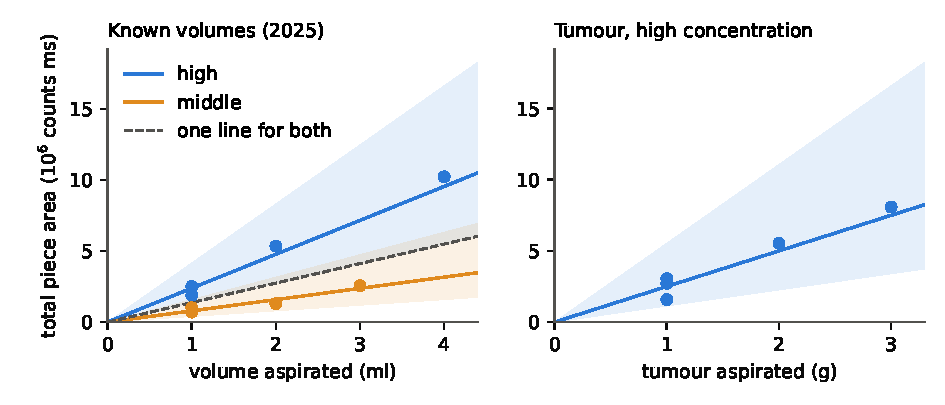
\includegraphics[width=\linewidth]{img/fig_amount.pdf}
  \caption{Total piece area of the first suction against the known amount. Lines: fitted $k$
           for each concentration; shaded: 95\,\% prediction interval for the first suction of a new recording;
           dashed: one $k$ for both.}
  \label{fig:amount}
\end{figure}

\begin{table}[H]
  \centering
  \caption{Mean error of the estimated amount (first suction, leave one recording out).
           $n$: number of recordings.}
  \label{tab:amount}
  \begin{tabular}{lrrrr}
    \toprule
    Recordings & $n$ & Count & Height\,$\times$\,width & Area \\
    \midrule
    Known volumes, high & 4 & 27\,\% & 28\,\% & 15\,\% \\
    Known volumes, middle & 4 & 46\,\% & 11\,\% & 21\,\% \\
    Tumour, high & 5 & 11\,\% & 19\,\% & 21\,\% \\
    Known volumes, concentration unknown & 8 & 32\,\% & 97\,\% & 68\,\% \\
    \bottomrule
  \end{tabular}
\end{table}

No concentration-free measure worked for both sets: area\,/\,height gave 19\,\% for the known
volumes but 46\,\% for the tumour, and the widths 31--71\,\%. Only the count was usable in both
(32\,\% and 11\,\%).

Compared with the known volumes (high), the tumour gives three times more pieces per unit amount
and half the peak height, but about the same area (\num{2.50e6} counts\,ms per gram vs
\num{2.39e6} per millilitre). The median peak width is \SI{12}{\milli\second} for the tumour and
28--\SI{30}{\milli\second} for the known volumes. At middle concentration, 10--27\,\% of the
signal above $3\sigma$ lies outside the events (high: 3--9\,\%). The threshold therefore matters
more for middle concentration: changing it from $10\sigma$ to $5\sigma$ or $20\sigma$ changes the
area of the first suction by at most 10\,\% at high concentration but by 6--23\,\% at middle
concentration (known volumes).

